\chapter{共識模組與系統架構}\label{se_5}

\section{共識模組}\label{se_5}
本章節介紹我們如何實作拜占庭容錯共識的架構。共識模組底下包含處理訊息的 Message Handler、同步訊息的 Synchronizer、與三個主要做共識的模組,Consensus Manager、Height Manager 與 Round Manager。共識模組間的關係如下圖。
\begin{figure}[h]
\centering
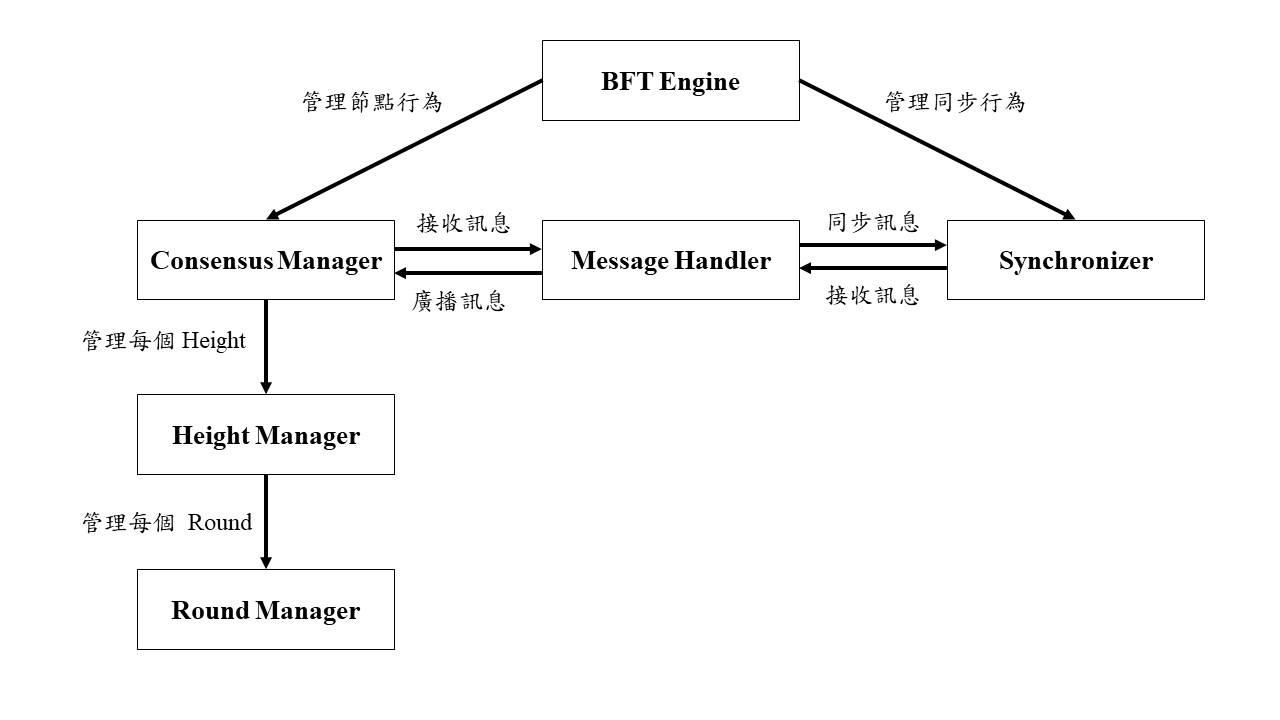
\includegraphics[scale=0.45]{images/5.jpg}
\caption{共識模組關係圖。}
\label{i:byz-latency}
\end{figure}
各共識模組之間相互負責不同事情。共識模組透過 go語言來進行實作,模組間參數時常共同管理(透過 go語言裡Channels來傳遞參數)。因此需要透過讀寫鎖,來控制讀寫流程,才不會造成多個模組同時讀寫情形。
。



\subsection{Consensus Manager}\label{se_5} 
Consensus Manager主要管理節點間連線,並且紀錄參與共識時所需的各式資訊,如:私有鏈ID、各節點地址、共識Timeout等等。
並且檢查區塊內的交易是否合法。Consensus Manager 核心技術在於定時的檢查自身狀態。如果滿足(一)廣播、(二)投票、(三)提交,任何一個狀態,則透過呼叫下層 Height Manager,進一步處理共識。同時也要將需要廣播的資訊交給 Message Handler。
\subsection{Height Manager}\label{se_5}
此模組主要功能是處理某一個高度的共識,透過管理一或多個 Round Manager 與其他節點溝通。(一)廣播:如果節點為該回合的Proposer且擁有前一回合票集合,呼叫下層 Round Manager 廣播新的共識提議;如果節點不是此回合的Proposer,等待新的共識提議被提出。(二)投票:呼叫Round Manager幫忙進行投票。(三)提交:確認高度是否已達成共識,如果還沒,則呼叫Round Manager進行提交共識。

\subsection{Round Manager}\label{se_5}
每個高度可能會需要一到多個回合,最終才能達成共識。因此Height Manager 可能須要建立多個 Round Manager 來進行共識。Round Manager 會蒐集來自 Height Manager 的訊息,經過判斷後採取對應動作。(一)廣播:對所有節點廣播共識提案、(二)投票:在一個回合裡,Round Manager只會對一個合法共識提案簽章並廣播。(三)提交:將區塊內容同步到自身資料庫,並進入下一個區塊高度。


\subsection{Message Handler}\label{se_5} 
Message handler 主要負責接收與廣播共識之中需要的訊息,在接收到來自其他節點的訊息時,進行判斷是否交給 Consensus Manager,或是過濾掉重複接受的訊息。

\subsection{Synchronizer}\label{se_5}
Synchronizer 主要目的為同步節點間訊息。因為網路間可能存在延遲,節點可能因此較晚進到共識,少了前面的訊息而無法執行共識。必須先與其他節點同步到最新狀態。  




\section{系統架構}\label{se_5}  
TwoStepBFT共識演算法相較於過去傳統三回合的共識演算法,能在網路傳輸穩定情況下,較快達成共識。我們的目標是測試TwoStepBFT在多個節點的私有鏈的效率,實驗將在AWS雲端伺服器上進行。為了達成這個目標,我們整合了許多自動化的開發套件來協助我們完成實驗。實驗系統架構主要如下圖所描述 

\begin{figure}[htbp]
\centering
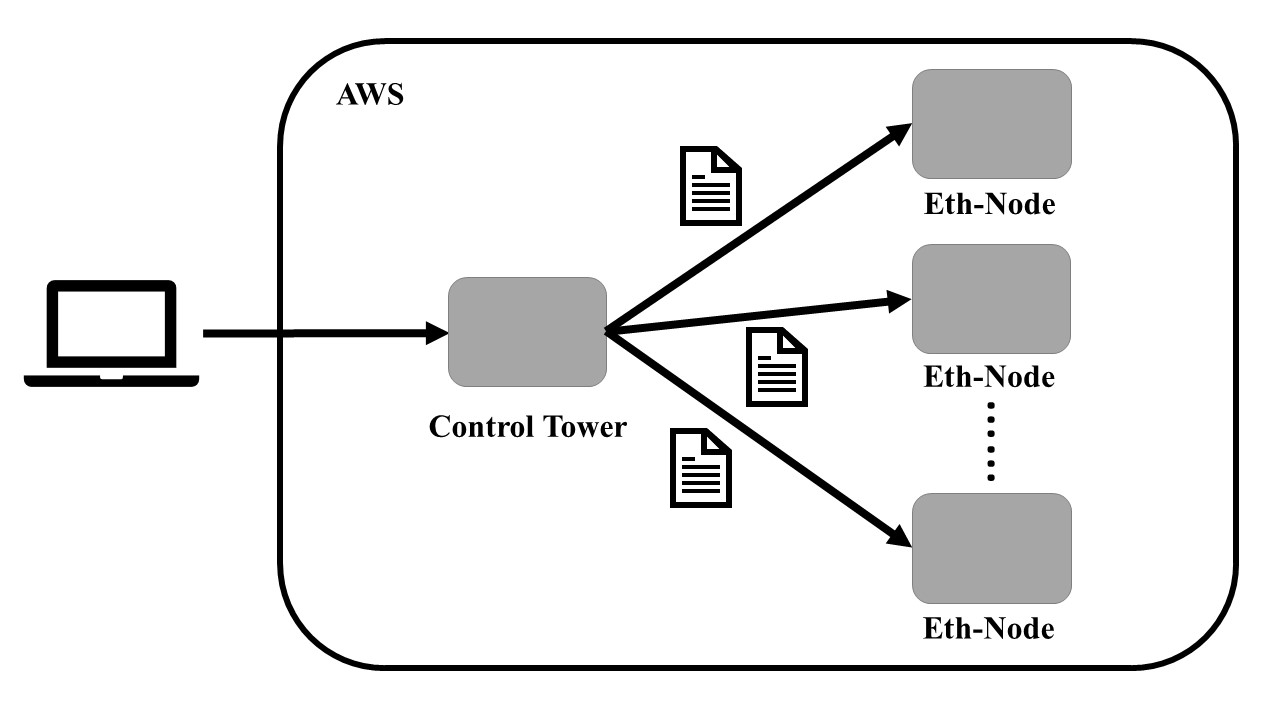
\includegraphics[scale=0.5]{images/51.jpg}
\caption{實驗系統架構圖。}
\label{i:byz-latency}
\end{figure}

該系統內含一個Control Tower,此台電腦類似實驗的中央控制中心,負責部署實驗環境到其他雲端機器上,並且收集其他機器所產生的實驗數據。該系統另包含數個區塊鏈節點,這些節點運行TwoStepBFT演算法,以達成區塊鏈共識。自動化多節點實驗主要分為兩大步驟: (1)高效率部署雲端系統 (2)自動化搭建私有鏈

\subsection{高效率部署雲端系統}\label{se_5} 
為了能夠在雲端平台上,快速開啟多台環境一致的機器,這些機器將成為區塊鏈的節點。我們整合了許多套件其中包含(一)Packer:能夠將實驗環境,打包成映像檔。這些映像黨裡會包含TwoStepBFT共識專案以及程式需要的各試工具。(二)Terraform:能夠依照使用者需求,動態產相對應的機器。
\begin{itemize}%项目符号开始
\item [1)] Packer: 為了能夠快速將上百個區塊鏈節點環境建立起來,因此使用了Hashicorp Packer這套工具來打包 AWS的AMI (Amazon Machine Images),AMI 能幫助我們快速建立出環境一致的節點。
Packer的優點如下

\item 極快速的部署:因為已經把需要的套件及其他設定都放在映像檔中,所以馬上可用。

\item 跨平台且可攜性:Packer 可針對不同平台打包出完全相同的映像檔,可在本地、雲端等各種不同平台獲得相同的運行環境。

\item 較好的測試性:映像檔一打包完成就可進行各種測試。

\item [2)] Terraform: Terraform能夠快速將AWS環境架設起來,依照使用者所撰寫程式碼搭建出所描述的架構,Terraform好處是能徹底實現基礎架構即代碼IaC (Infrastructure as code),利用代碼來配置實驗環境,讓環境安全且方便管理。
Terraform的優點如下:
\item   將基礎架構使用語法進行描述,可讓建構計劃像一般程式碼一樣進行版本控管與追蹤。 

\item Terraform會自動分析本地端計劃與遠端是否一至,自動化修改從而避免許多可能的人為操作錯誤。

\subsection{自動化搭建私有鏈}\label{se_5} 
為了讓我們快速搭建私有鏈,我們將搭建私有鏈步驟自動化。Go-ethereum 搭建私有鏈大致分為以下步驟(一)規劃私有鏈節點地址、IP地址、節點公私鑰。(二)依照使用者需求創造出Genesis.json,個節點可依照Genesis.json產生符合共識的節點。(三)將各節點產生的節點資訊回傳給Control Tower整合Static-node.json,並發送回給各節點,讓私有鏈呈現P2P網狀連線,此目的是為了能讓各節點彼此連接。

\begin{figure}[H]
\centering
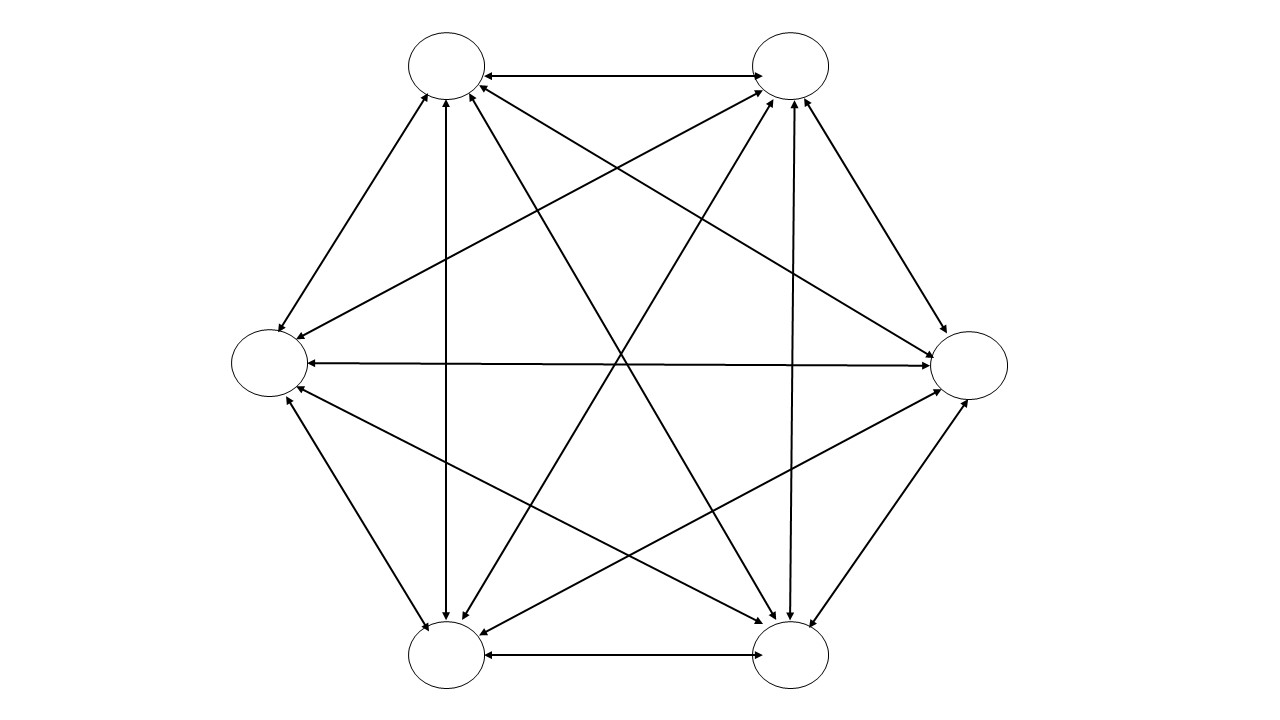
\includegraphics[scale=0.25]{images/6.jpg}
\caption{網狀連線範例圖。}
\label{i:byz-latency}
\end{figure}
\item [1)] Ethereum Wallet api: 系統環境建立後我們將透過Control Tower 動態產生實驗所需節點資訊,在我們的 實驗裡透過Ethereum Wallet api 動態的自動產生與實驗所需節點數之節點資訊(Public key, Address等等)

\item [2)] Genesis.json: Genesis.json 裡定義了區塊鏈資訊(包含區塊大小,區塊ID, 鏈上節點初始以太幣),由於每次實驗所產生節點帳戶地址都不相同,故我們將Genesis.json 設計成自動化動態產生,以方便實驗進行。 

\item [3)]Eth-client: 在Eth-client裡我們會執行節點間相互交易,Eth-client幫助我們每秒產生數百筆交易,鏈上的節點才能打包這些交易成為候選區塊,故與Genesis.json 相同因每次實驗所產生節點帳戶地址都不相同,我們也將Eth-client設計成自動化動態產生。 

\item [4)] Ansible: Ansible能幫助我們定義系統上的角色,方便我們依照不同角色執行相對應動作(ex. Control Tower會推送執行檔給鏈上節點執行,鏈上節點將實驗結果回傳至Control Tower做實驗分析。)

Ansible的優點如下:

\item 輕量級套件,無需在客戶端安裝agent,更新時,只需在操作機上進行一次更新即可。

\item 可將任務寫成腳本批次執行。

\item 使用python編寫,維護更簡單 。
\end{itemize}